\documentclass[11pt,a4paper]{ctexart}
\usepackage[margin=2.3cm]{geometry}
\usepackage{graphicx}
\usepackage{booktabs}
\usepackage{tabularx}
\usepackage{array}
\usepackage{float}
\usepackage{caption}
\usepackage{subcaption}
\usepackage{enumitem}
\usepackage{xcolor}
\usepackage{hyperref}
\usepackage{fancyhdr}
\usepackage{titlesec}
\usepackage{amsmath}

\hypersetup{
  colorlinks=true,
  linkcolor=black,
  urlcolor=blue,
  citecolor=black
}

\pagestyle{fancy}
\setlength{\headheight}{13.6pt}
\fancyhf{}
\lhead{大气缪子实验脱敏报告}
\rhead{装置搭建与数据分析}
\cfoot{\thepage}

\titleformat{\section}{\large\bfseries}{\thesection}{0.8em}{}
\titleformat{\subsection}{\normalsize\bfseries}{\thesubsection}{0.8em}{}
\setlist[itemize]{itemsep=2pt, topsep=3pt}
\setlist[enumerate]{itemsep=2pt, topsep=3pt}
\renewcommand{\arraystretch}{1.18}
\captionsetup{font=small, labelfont=bf}

\title{\textbf{大气缪子实验：从探测装置搭建到数据分析}}
\date{2025 年暑期科研实践整理}

\begin{document}
\maketitle
\thispagestyle{empty}

\begin{abstract}
本报告整理了一次大气缪子探测与数据分析实践。项目围绕桌面级缪子探测器展开，内容包括探测装置搭建、主从探测器符合模式理解、事件时间序列分析、每秒事件数泊松拟合、相邻事件时间间隔指数拟合，以及 SiPM 峰值电压谱比较。为便于公开展示，本报告仅保留方法、图表和阶段性结果，不公开原始数据、完整代码及个人身份信息。实验结果显示，候选事件在短时间计数上可用泊松过程近似描述，相邻事件时间间隔可用指数分布近似描述；主从符合筛选能够压低部分低电压背景，约 18.0 mV 的 SiPM 电压截断可作为一个经验筛选点。由于实验几何、背景抑制和标定条件有限，报告将结果表述为大气缪子候选事件分析，而不做逐事件粒子身份确认。
\end{abstract}

\vspace{0.8em}
\noindent\textbf{关键词：} 大气缪子；宇宙线；塑料闪烁体；SiPM；主从探测器；ROOT；泊松分布；指数分布

\newpage
\tableofcontents
\newpage

\section{项目背景}

宇宙射线是来自外太空的高能粒子流，主要成分包括质子和较重原子核。当这些高能粒子进入地球大气层后，会与氧、氮等大气分子发生核相互作用，产生一系列次级粒子。带电介子衰变后可产生缪子，部分高能缪子由于相对论时间膨胀和较强穿透能力，可以到达地面并被探测器记录。

大气缪子实验适合作为本科阶段粒子物理与实验数据分析训练的切口。一方面，它涉及宇宙线、粒子衰变、闪烁探测、光电转换和统计过程等基础物理概念；另一方面，实验链条相对完整，从装置搭建、信号采集到数据分析都可以亲手完成。与只在纸面上学习公式不同，这类实验需要把微弱、随机且带背景的自然信号转化为可分析的数据，再用统计模型判断观测是否与物理预期一致。

本项目使用桌面级缪子探测装置，对大气缪子候选事件进行初步观测和统计分析。项目目标不是完成高精度粒子鉴别，而是训练以下能力：

\begin{itemize}
  \item 理解闪烁体与 SiPM 的基本探测原理；
  \item 搭建并使用主从探测器模式进行符合筛选；
  \item 使用 Python 与 ROOT 完成基础数据处理和可视化；
  \item 用泊松分布和指数分布分析随机事件过程；
  \item 识别实验局限，并提出后续改进方向。
\end{itemize}

\section{实验装置与探测原理}

\subsection{探测器基本构成}

实验探测单元主要由塑料闪烁体、硅光倍增管（SiPM）、前端电子学和微控制器数据记录模块组成。原始实验记录中使用的探测单元包含塑料闪烁体和 SiPM。粒子穿过闪烁体时会沉积能量，引发闪烁光；闪烁光到达 SiPM 光敏面后触发微单元的盖革放电，产生电信号。经过放大和整形后，信号可由微控制器读取并记录。

每个事件记录通常包含以下信息：

\begin{itemize}
  \item 事件编号；
  \item 事件时间戳；
  \item ADC 峰值；
  \item 由 ADC 换算得到的 SiPM 峰值电压；
  \item 探测器死时间；
  \item 温度信息。
\end{itemize}

其中，SiPM 峰值电压可以作为信号强度的一个粗略表征。它并不等同于粒子能量的精确测量，但可以用于观察低电压背景、筛选候选事件和比较不同探测器通道的响应差异。

\subsection{主从探测器符合模式}

单个桌面探测器会对所有超过软件阈值的脉冲触发记录，因此可能包含自然放射性、电磁背景、电子学噪声等非目标成分。为了提高候选缪子事件的可信度，本项目引入 master/slave 主从探测器模式。

在该模式下，master 探测器记录所有超过阈值的事件；slave 探测器只在 master 探测器记录事件后的短时间窗口内也探测到信号时记录事件。本项目采用的符合窗口为约 15 微秒。由于随机背景事件同时触发两台探测器的概率较低，符合模式可以提升候选样本纯度。

需要注意的是，符合筛选提高的是候选事件的可信度，而不是逐事件的绝对确认。桌面级探测器对不同电离辐射形式均可能有响应，因此后续结论应保持审慎。

\section{数据处理方法}

本项目的数据分析部分使用 Python 与 ROOT / PyROOT 完成。公开报告不包含完整代码和原始数据，仅描述分析流程与核心结果。

\subsection{数据预处理}

数据预处理包括：

\begin{enumerate}
  \item 分别读取 master 与 slave 的记录文件；
  \item 提取事件时间戳与 SiPM 峰值电压；
  \item 去除明显无效或空白记录；
  \item 根据事件时间戳构造事件时间序列；
  \item 根据 SiPM 峰值电压构造电压谱。
\end{enumerate}

\subsection{每秒事件数与泊松拟合}

将事件时间戳按秒分箱，得到每秒事件数序列。若在短时间内事件可以近似看作独立随机到达过程，那么单位时间事件数应接近泊松分布：

\begin{equation}
P(k;\lambda)=\frac{\lambda^k e^{-\lambda}}{k!},
\end{equation}

其中 $k$ 表示每秒记录到的事件数，$\lambda$ 表示平均每秒事件数。分析中对每秒事件数频率直方图进行泊松拟合，并检查拟合结果是否与随机事件过程相符。

\subsection{相邻事件时间间隔与指数拟合}

若事件到达服从泊松过程，则相邻事件时间间隔 $\Delta t$ 应接近指数分布：

\begin{equation}
f(\Delta t;\tau)=\frac{1}{\tau}\exp\left(-\frac{\Delta t}{\tau}\right),
\end{equation}

其中 $\tau$ 是平均时间间隔，计数率可近似写为 $r=1/\tau$。本项目分别对 master、slave 以及经过电压阈值筛选后的数据进行时间间隔统计和指数函数拟合。

\subsection{SiPM 电压谱与阈值筛选}

SiPM 峰值电压谱用于观察不同强度信号的分布。通过比较 master 与 slave 的电压谱，可以看到低电压区域的事件在符合筛选后显著减少，说明这一区域可能包含较多背景或非目标触发。

为进一步提升筛选后数据的信噪比，分析中尝试寻找经验电压截断点。根据大于截断电压部分的 slave 与 master 信号量比例变化，选取约 18.0 mV 作为初步截断阈值，并对截断后的数据重新进行时间间隔分析。

\section{分析结果}

\subsection{每秒事件数分布}

图 \ref{fig:event_analysis} 展示了 slave 数据的事件时间分布和每秒事件数频率分布。拟合结果给出 $\lambda\approx 1.39$，$\chi^2/\mathrm{NDF}\approx 1.94$。这一结果说明，在本实验时间尺度和探测条件下，每秒事件数可用泊松分布进行近似描述。

\begin{figure}[H]
  \centering
  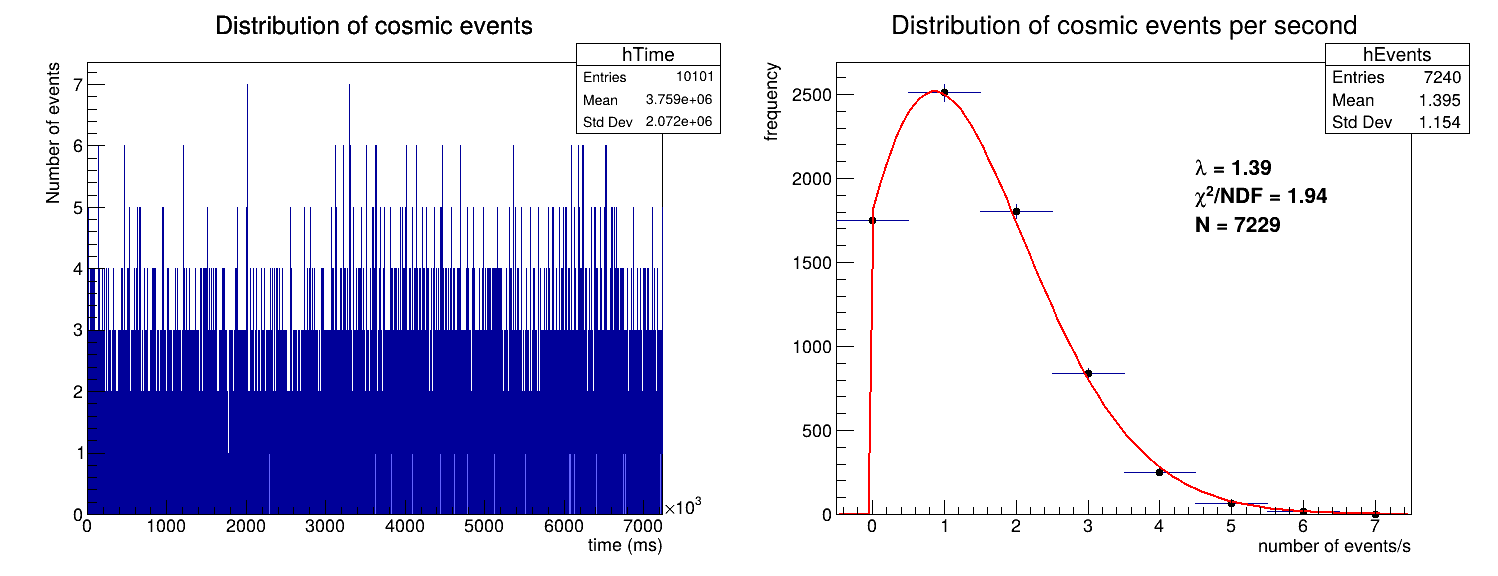
\includegraphics[width=0.95\linewidth]{../figures/event_analysis.png}
  \caption{事件时间分布与每秒事件数泊松拟合。右图显示每秒记录到的事件数频率分布，红线为泊松拟合曲线。}
  \label{fig:event_analysis}
\end{figure}

\subsection{事件时间间隔分布}

图 \ref{fig:interval_master_slave} 展示了 master 与 slave 数据的相邻事件时间间隔分布。master 数据总事件数为 35822，平均间隔约 203.0 ms，计数率约 4.93 Hz；指数拟合得到 $\tau'\approx203.33 ms$。slave 数据总事件数为 10101，平均间隔约 716.8 ms，计数率约 1.40 Hz；指数拟合得到 $\tau'\approx702.77 ms$。

master 计数率高于 slave，符合主从模式的预期：master 记录所有超过阈值的触发，slave 只保留与 master 符合的事件，因此样本数显著减少。

\begin{figure}[H]
  \centering
  \begin{subfigure}{0.49\linewidth}
    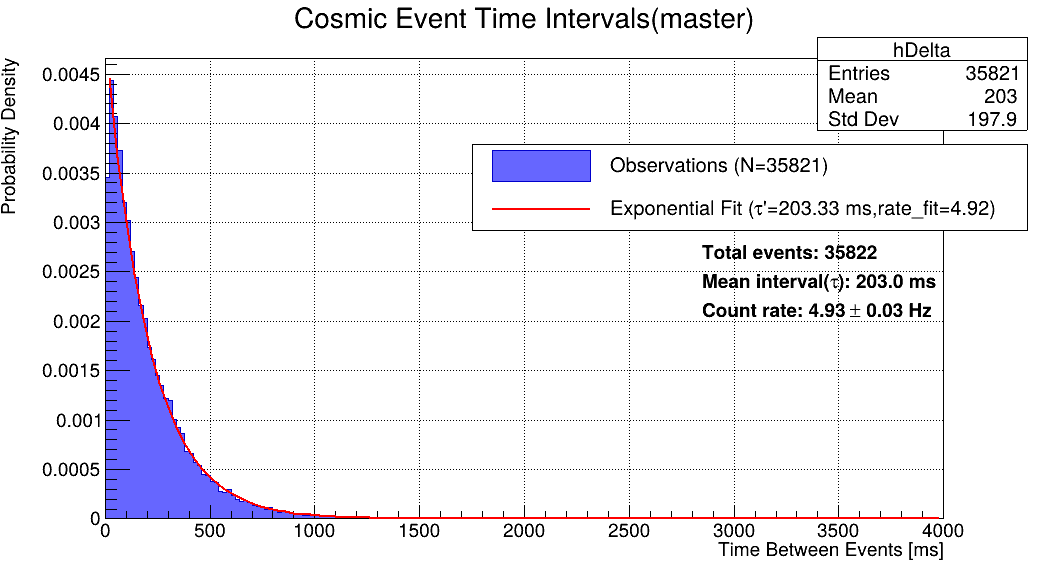
\includegraphics[width=\linewidth]{../figures/time_intervals_master.png}
    \caption{master 相邻事件时间间隔}
  \end{subfigure}
  \hfill
  \begin{subfigure}{0.49\linewidth}
    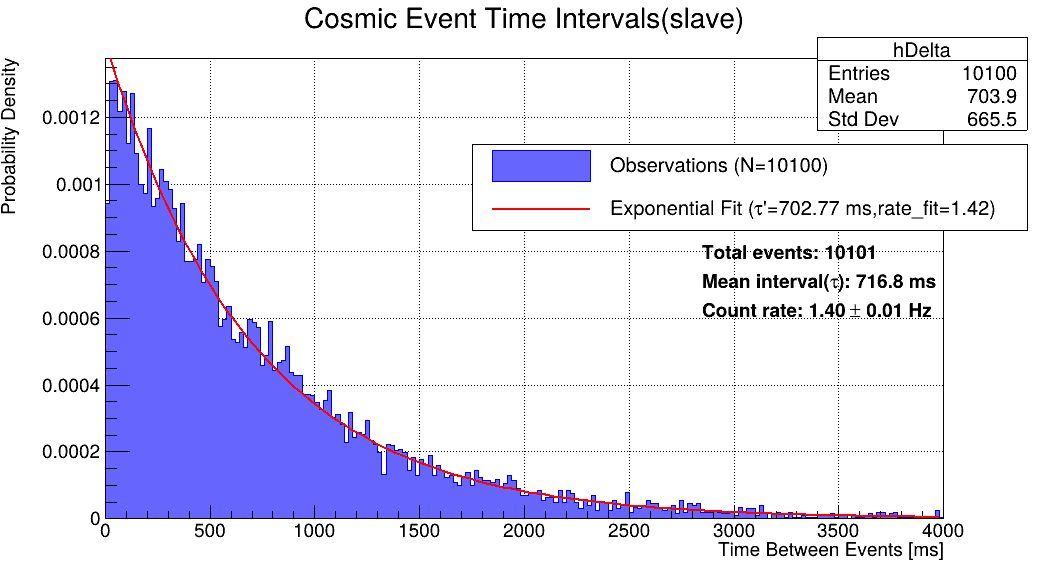
\includegraphics[width=\linewidth]{../figures/time_intervals_slave.png}
    \caption{slave 相邻事件时间间隔}
  \end{subfigure}
  \caption{相邻事件时间间隔的指数分布拟合。红线为指数拟合曲线。}
  \label{fig:interval_master_slave}
\end{figure}

\subsection{SiPM 电压谱比较}

图 \ref{fig:voltage_spectrum} 展示了 master 与 slave 的 SiPM 峰值电压谱。master 记录事件数为 35822，均值约 16.53 mV；slave 记录事件数为 10101。低电压区域 master 事件明显更多，而 slave 由于要求符合触发，低电压背景被明显压低。

\begin{figure}[H]
  \centering
  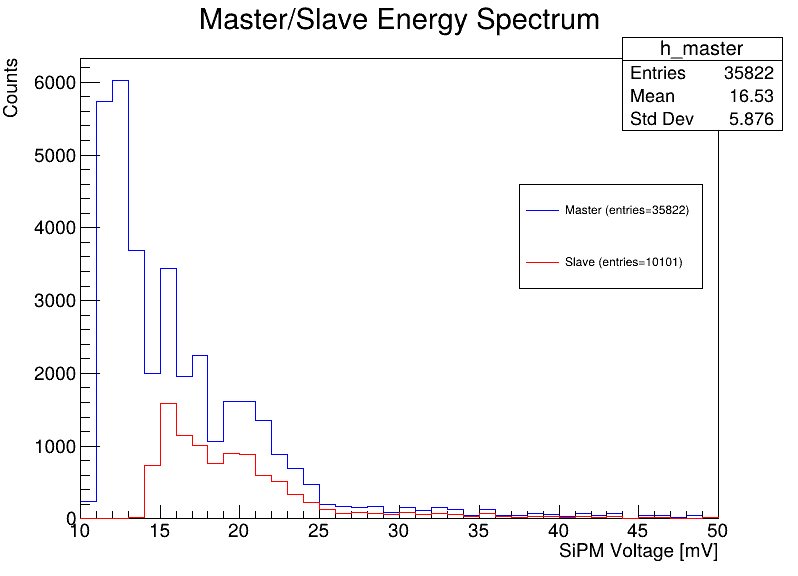
\includegraphics[width=0.82\linewidth]{../figures/master_vs_slave.png}
  \caption{master 与 slave 的 SiPM 峰值电压谱。蓝色为 master，红色为 slave。}
  \label{fig:voltage_spectrum}
\end{figure}

图 \ref{fig:comparison_diff} 进一步展示了 master、slave 及二者差异的电压分布。差异主要集中在较低电压区，说明这一区间可能包含较多未通过符合筛选的触发事件。

\begin{figure}[H]
  \centering
  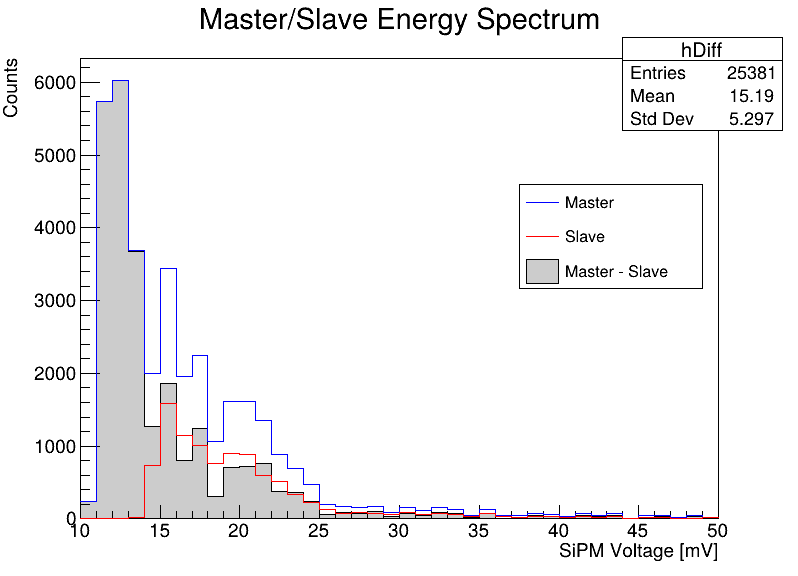
\includegraphics[width=0.82\linewidth]{../figures/comparison_diff.png}
  \caption{master / slave 电压谱差异。灰色区域表示 master 相对 slave 的差异计数。}
  \label{fig:comparison_diff}
\end{figure}

\subsection{电压阈值截断后的时间间隔分布}

根据电压谱分析，本项目尝试采用约 18.0 mV 的电压截断对事件进行筛选。图 \ref{fig:interval_cut} 展示了截断后的 master 与 slave 时间间隔分布。截断后，master 数据总事件数约 10489，平均间隔约 693.3 ms，计数率约 1.44 Hz；slave 数据总事件数约 5602，平均间隔约 1292.3 ms，计数率约 0.77 Hz。

截断会减少事件数，同时使保留样本更偏向较高电压触发。该结果可作为后续优化筛选策略的起点，但阈值本身仍属于经验选择，需要通过更多对照实验和效率标定进一步验证。

\begin{figure}[H]
  \centering
  \begin{subfigure}{0.49\linewidth}
    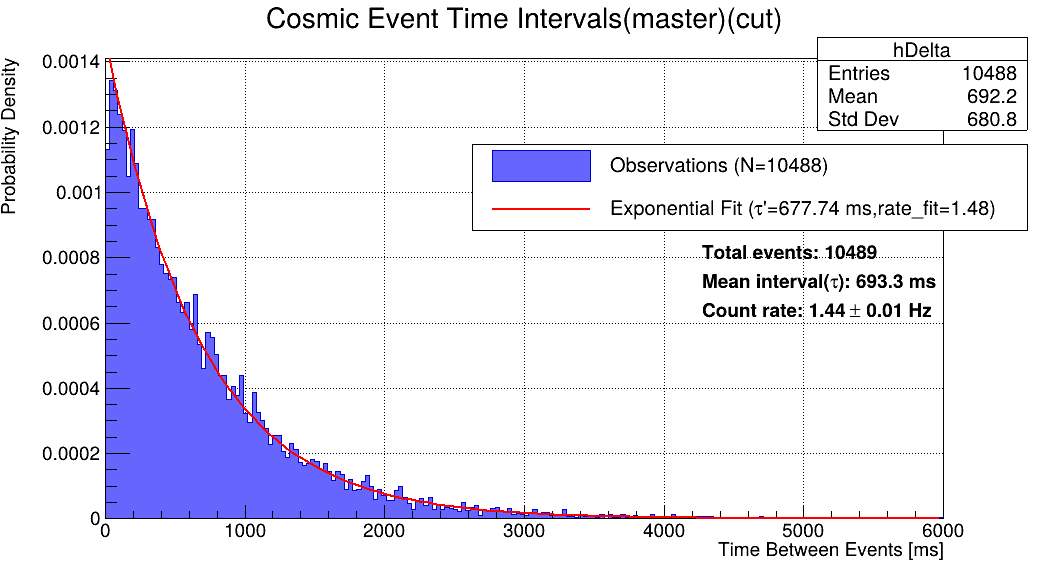
\includegraphics[width=\linewidth]{../figures/time_intervals_master_cut.png}
    \caption{master 电压截断后}
  \end{subfigure}
  \hfill
  \begin{subfigure}{0.49\linewidth}
    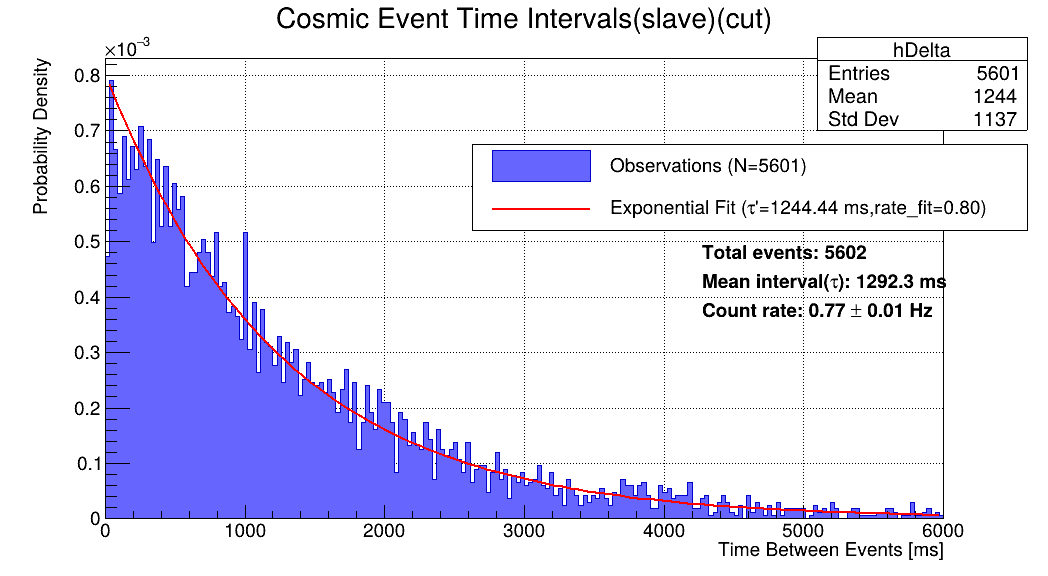
\includegraphics[width=\linewidth]{../figures/time_intervals_slave_cut.png}
    \caption{slave 电压截断后}
  \end{subfigure}
  \caption{电压阈值筛选后的相邻事件时间间隔分布。}
  \label{fig:interval_cut}
\end{figure}

\section{结果汇总与讨论}

\begin{table}[H]
\centering
\caption{主要统计结果汇总}
\begin{tabularx}{\linewidth}{>{\raggedright\arraybackslash}p{3.3cm}>{\raggedright\arraybackslash}X>{\raggedright\arraybackslash}p{3.5cm}}
\toprule
分析对象 & 主要结果 & 物理或方法含义 \\
\midrule
每秒事件数 & $\lambda\approx 1.39$，$\chi^2/\mathrm{NDF}\approx 1.94$ & 事件计数可近似看作随机到达过程 \\
master 时间间隔 & 平均间隔约 203.0 ms，计数率约 4.93 Hz & master 保留所有超过阈值的触发，计数率较高 \\
slave 时间间隔 & 平均间隔约 716.8 ms，计数率约 1.40 Hz & 符合筛选后事件数减少，样本可信度提高 \\
SiPM 电压谱 & 低电压区 master 与 slave 差异显著 & 低电压区可能有较多背景或非目标触发 \\
电压阈值截断 & 约 18.0 mV 可作为经验筛选点 & 可用于初步压低低电压背景，但需进一步标定 \\
\bottomrule
\end{tabularx}
\end{table}

整体来看，本项目完成了从装置建立、数据读取、统计建模到结果解释的闭环，并把实验信号放进统计框架中理解：若事件是随机到达的，短时间计数应接近泊松分布，相邻事件间隔应接近指数分布；若符合筛选有效，slave 相对于 master 的低电压背景应被压低。

\section{局限性与后续工作}

本项目仍有明显局限：

\begin{itemize}
  \item \textbf{粒子身份确认有限：} 由于桌面级探测器对多种电离辐射均可能响应，单凭本实验数据不能逐事件严格判定信号均为大气缪子。
  \item \textbf{几何接受度未充分标定：} 主从探测器的相对位置、角度和间距会影响符合事件的几何接受度。
  \item \textbf{环境因素未系统分析：} 温度、气压和实验场地背景可能影响计数率，目前尚未做长期环境变量关联。
  \item \textbf{阈值选择仍偏经验：} 18.0 mV 截断点来自本轮数据的经验观察，后续需要结合效率、纯度和对照实验优化。
\end{itemize}

后续可以从以下方向改进：

\begin{enumerate}
  \item 做不同探测器间距和角度下的符合计数率测量；
  \item 引入屏蔽材料对照，观察低能背景的变化；
  \item 进行更长时间采集，分析气压、温度等环境变量对计数率的影响；
  \item 尝试角分布测量，检验缪子通量随天顶角变化的趋势。
\end{enumerate}

\section{结论}

本项目以大气缪子候选事件为对象，完成了探测器原理理解、装置搭建参与、主从符合筛选、事件计数统计、时间间隔拟合和电压谱分析等工作。实验结果表明，候选事件在短时间计数和相邻事件间隔上具有随机过程特征，主从符合模式可以减少低电压背景，电压阈值筛选能够进一步改变保留事件的统计特征。

更重要的是，这一项目提供了一个完整的实验训练场景：一个物理问题不是从公式直接跳到答案，而是经过装置、信号、数据、统计模型和局限性判断一步步展开。对于本科阶段科研项目而言，这比单纯得到一个漂亮结论更有价值。

\section*{参考资料}
\addcontentsline{toc}{section}{参考资料}

\begin{enumerate}[label={[\arabic*]}]
  \item Spencer N. Axani. \textit{The Physics Behind the CosmicWatch Desktop Muon Detectors}. 2018.
  \item T. K. Gaisser, R. Engel, and E. Resconi. \textit{Cosmic Rays and Particle Physics}. Cambridge University Press, 2016.
  \item M. G. Aartsen et al. \textit{The IceCube Neutrino Observatory: Instrumentation and Online Systems}. Journal of Instrumentation, 2017.
  \item K. Morishima et al. \textit{Discovery of a big void in Khufu's Pyramid by observation of cosmic-ray muons}. Nature, 2017.
  \item Z. Cao et al. \textit{Introduction to the Large High Altitude Air Shower Observatory}. Chinese Astronomy and Astrophysics, 2019.
\end{enumerate}

\end{document}
